% Diseño Analógico. Introducción, características de las señales 
% según el estándar, arquitectura del circuito, acondicionamiento de 
% la energía (rectificadores, regulador, Iref), detector de 
% envolvente, extracción de reloj y POR. Simulaciones, mediciones. 
\chapter{Diseño Analógico}

En este capítulo se realizará un recorrido por los bloques 
analógicos del circuito integrado. El diseño analógico comprende 
cuatro sistemas que hacen de soporte al bloque digital y que se 
verán a continuación. El primero de ellos es el sistema de captura y 
acondicionamiento de la energía, que debe tomar la energía recibida 
a través de la señal portadora, almacenarla y acondicionarla para 
ser usada por los demás bloques del circuito integrado. En segundo 
lugar se verá el sistema de transmisión y recepción de datos, que 
por un lado se encarga de demodular la señal enviada por el lector y 
adaptarla a los niveles lógicos del bloque digital; y por otro 
realiza la modulación de carga sobre la señal portadora para 
transmitir hacia el lector. Luego se verá el sistema de captura y 
reconstrucción de la señal de reloj a partir de la portadora de 
\SI{13.56}{\mega\hertz} y para finalizar se analizará el 
\emph{power-on reset}, que inicializa la lógica digital a través de la 
señal \lstinline{reset} cuando la tensión de alimentación alcanza el 
nivel de operación.


\section{Acondicionamiento y uso de la energía}

Como se vio en la sección \ref{sec:TransmisionDeLaEnergia} la amplitud 
de la tensión en la antena varía con la distancia entre el lector y 
el transponder durante la operación normal del dispositivo. Por este 
motivo es que se implementó el bloque <<Regulador/Limitador de 
tensión>>, que tiene como objetivo mantener la tensión a la entrada 
de la antena dentro del nivel de funcionamiento a pesar de las 
variaciones de la distancia al lector o, lo que es lo mismo, las 
variaciones en el coeficiente de acoplamiento. Para lograrlo la idea 
es cargar a la antena con una carga interna dentro del transponder 
de forma tal de cancelar las variaciones de amplitud 
debidas a los cambios en el coeficiente de acoplamiento. 

Por otra parte se debe tomar la tensión alterna generada en la antena, 
rectificarla y filtrarla para ser usada como tensión de alimentación 
dentro del chip. Esto se hace con el bloque <<Rectificador + Filtro>> 
de la figura \ref{fig:DiagramaEnBloquesCI}. Entonces se tiene por un 
lado el regulador de tensión que actúa de carga variable, y por otro la
toma de energía a través del bloque <<Rectificador + Filtro>>, ambos 
conectados a la entrada de la antena.

\subsection{Regulador/Limitador de tensión}

Se trata de un regulador de tensión de tipo paralelo y la idea es 
ajustar una carga variable de forma tal de regular la tensión 
inducida en la antena, manteniéndola por debajo del límite de 
tensión máxima permitida por el proceso de fabricación CMOS.

En la figura \ref{fig:ReguladorCircuito} se muestra el regulador 
propuesto. La tensión alterna de la antena en los nodos \(rf_{1}\) y 
\(rf_{2}\) es convertida mediante el rectificador de onda completa a 
tensión continua en el nodo \(V_{reg}\). A la salida del 
rectificador se encuentra conectada la carga variable, que fue 
implementada con un transistor NMOS, y es controlada por la señal de 
error que produce el amplificador diferencial. La señal de error 
surge de amplificar la diferencia de tensión entre la tensión de 
referencia \( V_{gn}\) y una muestra de la tensión \(V_{reg}\). La 
tensión de referencia es tomada de la referencia de corriente, que 
es de tipo \emph{Beta Multiplier} \cite{Baker}.

\begin{figure}
	\centering
	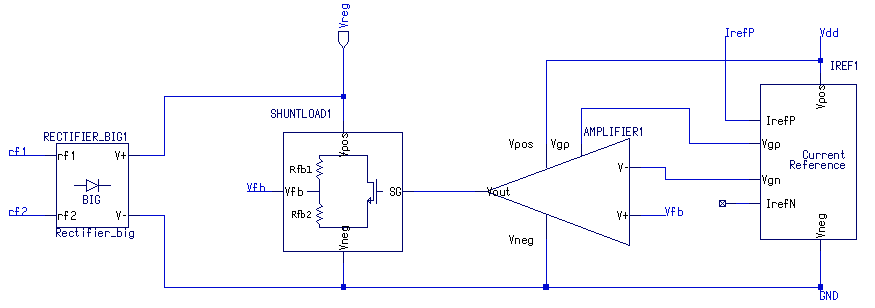
\includegraphics[width=\columnwidth]{Regulador_circuito}
	\caption{Circuito Regulador/Limitador de tensión.}
	\label{fig:ReguladorCircuito}
\end{figure}

La tensión \(V_{reg}\) es una onda senoidal rectificada y por lo tanto 
varía en función del tiempo con el doble de frecuencia que la señal 
portadora, es decir, \SI{27.12}{\mega\hertz}. El lazo de 
realimentación debe ser lo suficientemente lento como para no reaccionar 
ante las variaciones de amplitud instante a instante, sino al valor 
medio de la señal, que es \(\sfrac{2 V_{p}}{\pi}\), donde 
\(V_{p}\) es el valor pico. 

En la figura \ref{fig:Rectificador} se muestra el circuito del 
rectificador. Está formado por cuatro transistores NMOS, dos 
conectados como diodos y dos con los gates cruzados. Esta topología se 
eligió por sobre otras debido a que su rendimiento es mejor que el de 
un rectificador con cuatro en NMOS o PMOS, como se analiza extensamente en 
\cite{RectifierComparison}, y además es una topología simple y de 
fácil implementación. 

\begin{figure}
	\centering
	\begin{subfigure}[b]{0.45\textwidth}
		\centering
		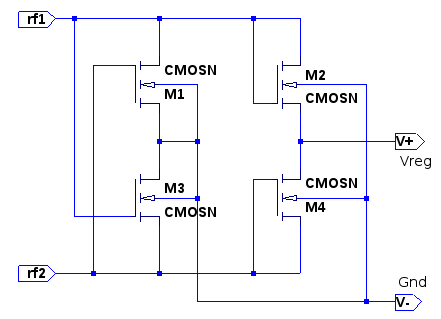
\includegraphics[width=\columnwidth]{Rectificador}
		\(\scriptstyle\mathrm{M1,M3: \frac{W}{L}}= 
		\frac{\SI{105}{\micro\meter}}{\SI{0.6}{\micro\meter}};\;
		\mathrm{M2,M4: 
		\frac{W}{L}}=\frac{\SI{210}{\micro\meter}}{\SI{0.6}{\micro\meter}}\)
		\caption{Esquemático}
		\label{fig:Rectificador}
	\end{subfigure}
	\quad
	\begin{subfigure}[b]{0.45\textwidth}
	    \centering
		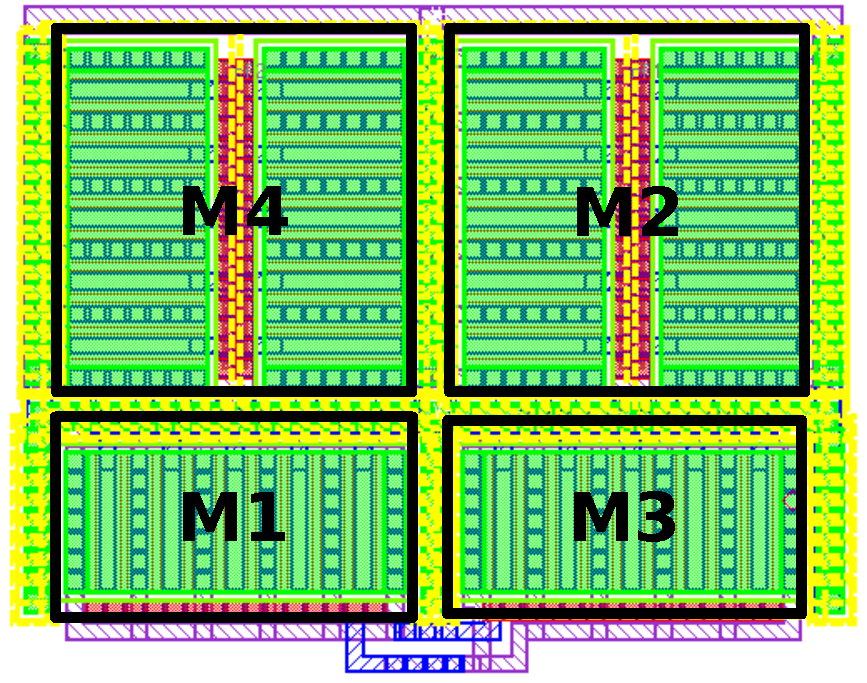
\includegraphics[width=\columnwidth]{Layout_Rectificador.pdf}
		\caption{Layout}
		\label{fig:LayoutRectificador}
	\end{subfigure}
	\caption{Esquema del rectificador y su trazado físico.}
	\label{fig:RectificadorYLayout}
\end{figure}

La tensión máxima que se puede tener a la entrada del circuito 
integrado está limitada por la tensión máxima admisible a la entrada 
del rectificador, ya que las tensiones \(V_{gs}\) de M1 y M3 son 
iguales a la tensión de la antena y no pueden superar los 
\SI{5.5}{\volt} máximos del proceso.

Según la figura \ref{fig:TensionInducida}, para limitar la tensión 
inducida con campo máximo en una antena de \SI{8}{\micro\henry} a 
\SI{5.5}{\volt} se la debe cargar con \SI{360}{\ohm} aproximadamente. 
En estas condiciones el regulador de tensión deberá consumir 
\SI{15}{\milli\ampere} de corriente pico. Los transistores que están 
conectados como diodos en el rectificador (M2 y M4) fueron 
dimensionados para que con una corriente de esa magnitud la caída de 
tensión no sea mayor a \SI{1.5}{\volt}. Para ello, por simulación se 
trazó la curva \(I_{d}=f(V_{ds})\) de un transistor conectado de esa 
manera y se fue incrementando el ancho del canal hasta obtener los 
valores deseados.

El hecho de conectar los gates de M1 y M3 de forma cruzada permite 
tener una tensión \(V_{gs}\) mayor y por lo tanto una corriente de 
drain mayor, o lo que es lo mismo, igual corriente que M2 y M4 con 
un \(V_{ds}\) menor. Por otro lado, este par de transistores tienen 
conectados sus bulks, que están formados por el substrato de tipo P, 
al nodo GND y sus terminales de source a rf1 y rf2 respectivamente. 
Este conexionado posibilita que se ponga en directa la juntura 
bulk-source (bulk tipo P y source tipo N) en el retorno de la 
corriente. Sin embargo, cruzar los gates de los transistores evita 
que eso suceda ya que la tensión \( V_{ds}\) es menor que la tensión 
umbral de conducción de la juntura bluk-source.

En la figura \ref{fig:LayoutRectificador} se muestra el trazado físico 
del rectificador. Para evitar tener una corriente de 
\SI{15}{\milli\ampere} a través de un solo transistor se decidió 
dividir los dispositivos en varios transistores en paralelo. Así, M2 y 
M4 están compuestos por 20 NMOS en paralelo, lo que da un ancho de 
canal efectivo de \SI{210}{\micro\meter}, y M1 y M3 están compuestos por 
10 transistores resultando un ancho efectivo de \SI{105}{\micro\meter}.

\bigskip
Volviendo al circuito regulador de tensión, la amplitud de la 
tensión alterna en los nodos \(rf_{1}\) y \(rf_{2}\) está vinculada 
con la amplitud de la tensión \(V_{reg}\) a través de la caída de 
tensión en el rectificador, que puede considerarse de \SI{1.5}{\volt} 
en el peor de los casos. Además, la tensión máxima que se puede 
tener a la entrada es de \SI{5.5}{\volt}, entonces, se debe mantener 
la tensión \(V_{reg}\) por debajo de \SI{4}{\volt} para que, sumando 
la caída en el rectificador, la amplitud de la tensión en la antena 
no supere los \SI{5.5}{\volt}. Un valor pico de \SI{4}{\volt} en 
\(V_{reg}\) se tiene si se regula su valor medio a \SI{2.5}{\volt}, 
por lo tanto el lazo de realimentación debe mantener el valor medio por 
debajo de ese valor.

\begin{figure}
	\centering
	    \begin{subfigure}[b]{0.35\textwidth}
	    \centering
		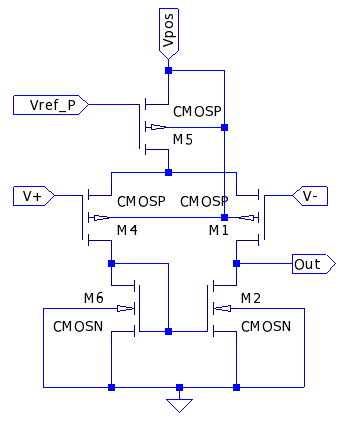
\includegraphics[width=\columnwidth]{Amplificador_LTSpice}
		\(\scriptstyle\mathrm{M1\text{-}M6: \frac{W}{L}}= 
		\frac{\SI{6}{\micro\meter}}{\SI{3}{\micro\meter}};\)
		\caption{Amplificador}
		\label{fig:Amplificador}
	\end{subfigure}
	\quad
	\begin{subfigure}[b]{0.35\textwidth}
	    \centering
		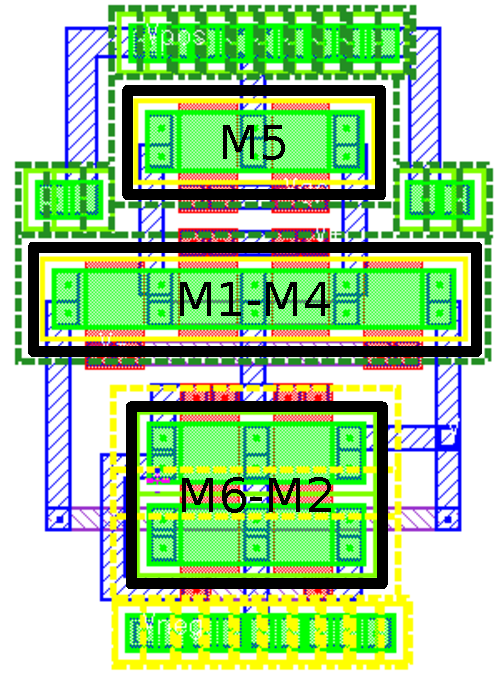
\includegraphics[width=\columnwidth]{Layout_amplifier.pdf}
		\caption{Layout}
		\label{fig:LayoutAmplificador}
	\end{subfigure}
	\caption{Esquema del amplificador y su trazado físico.}
	\label{fig:AmplificadorYLayout}
\end{figure}

La tensión de referencia de \SI{1}{\volt} se compara mediante el 
amplificador diferencial con la tensión \(V_{fb}\), resultante de 
\(V_{reg}\) aplicada a un divisor resistivo. El amplificador no es más 
que el par diferencial con carga activa de la figura 
\ref{fig:Amplificador} y su ganancia es de 100 veces. El ancho de banda 
del amplificador es de \SI{100}{\kilo\hertz} y está dado por la 
capacidad del gate del transistor de carga que, dada la corriente que 
debe manejar, es de tamaño similar a los del rectificador. La baja 
ganancia del par diferencial junto al bajo ancho de banda ayudan a 
mantener la estabilidad del lazo de realimentación, según se analiza 
en \cite{Gudnason}.

Además, en esta implementación la carga utilizada es de tipo 
resistiva y en principio puede afectar la transmisión de datos, que 
precisamente se realiza mediante modulación de carga. Como se 
observó en el análisis de la sección \ref{sec:InterfIndTransDatos}, 
en la figura \ref{fig:VsensModulacionR}, variar el valor de una 
carga resistiva cuando se tiene un circuito de antena de tipo RL 
produce una modulación de la tensión \(V_{sens}\) a la salida del 
arreglo de prueba. Sin embargo, el lector identifica los datos 
demodulando la sub-portadora y entonces, si la variación de la carga 
se realiza de forma lenta, a una velocidad mucho menor que la 
frecuencia de la sub-portadora, el lector no la detectará como 
transmisión de información. Este es otro motivo por el que es 
conveniente tener un ancho de banda reducido en el lazo de 
realimentación. 

Las resistencias en el lazo de realimentación se calcularon de forma 
tal de que con \SI{2.2}{\volt} de valor medio en \(Vreg\), \(V_{fb}\) 
sea igual a \(V_{ref}\), es decir que se cumpla:

\begin{equation*}
	\bar{V}_{fb} = \bar{V}_{reg} \frac{R_{fb2}}{R_{fb1}+R_{fb2}} = V_{ref}
\end{equation*}

Además, para evitar tener un consumo excesivo de corriente a través del 
divisor resistivo se eligieron \SI{120}{\kilo\ohm} y 
\SI{100}{\kilo\ohm} para \(R_{fb1}\) y \(R_{fb2}\) 
respectivamente.

\bigskip
En cuanto a la referencia de tensión, ésta se toma de la salida 
\(V_{tn}\) de la referencia de corriente de la figura 
\ref{fig:BetaMultiplierCircuito}. Allí los transistores M1 a M4 forman 
una referencia de corriente de tipo \emph{Beta Multiplier} \cite{Baker},
M5 a M8 conforman el circuito de arranque, necesario para evitar el punto 
estable de cero corriente, y M9 y M10 copian las corrientes de la 
referencia y las distribuyen a otros circuitos.

\begin{figure}
	\centering
	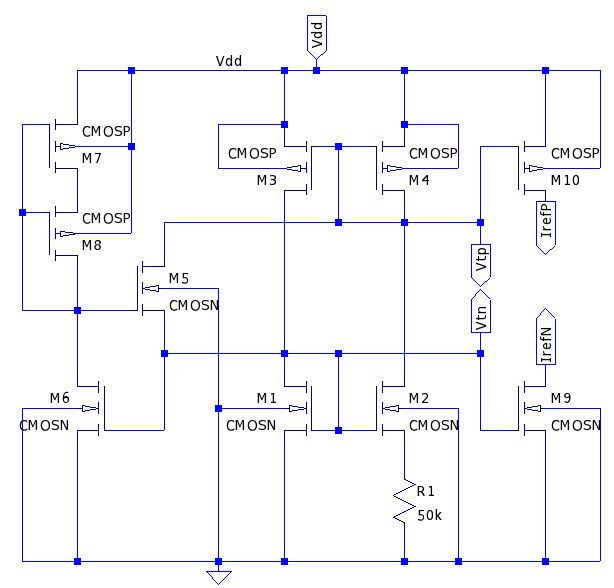
\includegraphics[width=0.6\columnwidth]{Iref_LTSpice}
	\caption{Referencia de corriente/tensión. M1 a M4 forman un 
	circuito \emph{Beta Multiplier}, M5 a M8 forman el circuito de 
	arranque y M9 y M10 copian la corriente para ser usada por otros 
	bloques. (M2 = 4M1 y M3 = M4)}
	\label{fig:BetaMultiplierCircuito}
\end{figure}

En la figura \ref{fig:BetaMultiplierLayout} se muestra el trazado 
físico de la referencia de corriente. Para evitar las variaciones 
entre transistores que deben ir apareados se los ubicó a todos en la 
misma orientación y se los dividió en tamaños iguales, ubicándolos 
de forma simétrica con respecto al centro del bloque. El resistor R1 
fue fabricado con \emph{poly2} con un implante que aumenta su 
resistencia por cuadrado a \SI{1}{\kilo\ohm} y se agregaron resistores 
extras en los extremos para evitar los efectos del acabado en los 
bordes.

\begin{figure}
	\centering
	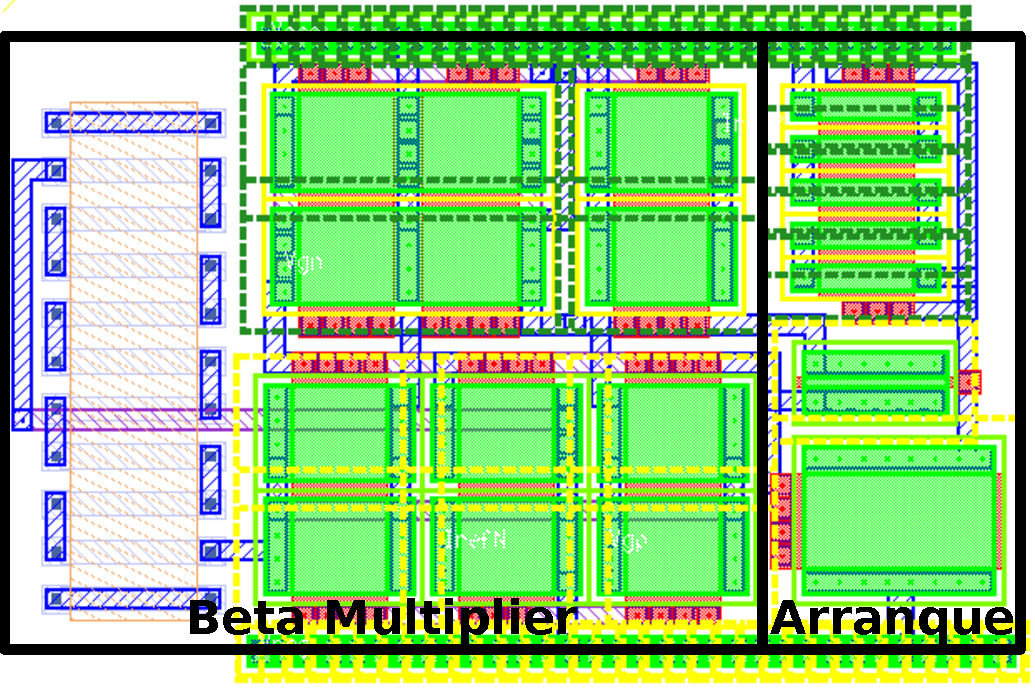
\includegraphics[width=0.6\columnwidth]{Layout_Iref.pdf}
	\caption{\emph{Layout} de la fuente de corriente con su circuito 
	de arranque.}
	\label{fig:BetaMultiplierLayout}
\end{figure}

La tensión de referencia no tiene grandes exigencias en 
cuanto a su valor absoluto ya que da lo mismo si el regulador limita 
el valor medio de \(V_{reg}\) a \SI{2}{\volt} o \SI{2.5}{\volt}, 
siempre y cuando no se pase de este último, debido a que el sistema 
digital funcionará de todas maneras. Es por eso que se decidió 
utilizar la tensión \(V_{tn}\), que si bien varía ligeramente con la 
tensión de alimentación y las variaciones del proceso, como se 
observa en la figura \ref{fig:BetaMultiplierSim}, su variación es de 
apenas \SI{50}{\milli\volt}.

\begin{figure}
	\centering
	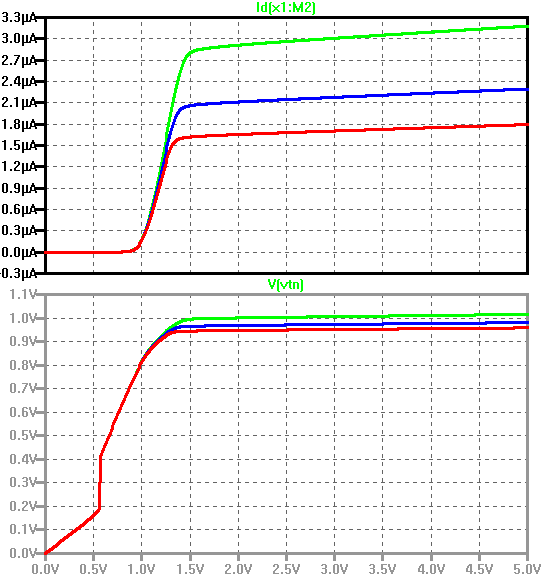
\includegraphics[width=0.6\columnwidth]{Iref_LTSpice_Sim}
	\caption{Simulación del \emph{Beta Multiplier} de la figura 
	\ref{fig:BetaMultiplierCircuito}. Las tres curvas corresponden a 
	variaciones del proceso de fabricación que pueden afectar el valor
	de \(R_{1}\) en un 20\%.}
	\label{fig:BetaMultiplierSim}
\end{figure}

La corriente del \emph{Beta Multiplier} se utiliza de referencia para 
crear copias con fuentes de corriente espejo en el par diferencial y 
en el circuito detector de pausas que se verá más adelante. Los 
transistores M1 a M4 tienen \SI{6}{\micro\meter} de largo para evitar 
los efectos de canal corto que aumentan la variación de \(I_{ref}\) 
con la tensión de alimentación \cite{Baker}.

\bigskip
En la figura \ref{fig:ReguladorSim} se muestran dos simulaciones del 
regulador en funcionamiento. Las simulaciones se realizaron 
conectando el regulador/limitador de tensión al modelo del arreglo 
de antenas de la figura \ref{fig:ArregloDeAntenasVista3D} y por la 
antena del PCD se hicieron circular corrientes tales que produzcan 
los campos máximo y mínimo de la norma en la posición de la antena 
del transponder. Para todos los dispositivos se utilizaron los valores 
nominales de diseño junto con el modelo de los transistores del
último proceso de fabricación.

Los gráficos superiores muestran la corriente que 
circula por el transistor de paso, que es la que sale del 
rectificador y por lo tanto tiene forma de onda senoidal rectificada. 
En los gráficos inferiores se muestra la tensión inducida en la antena 
(\(V(rf1,rf2)\)), la tensión en el transistor de paso (\(V_{reg}\)), 
la tensión de referencia (\(V_{ref}\)) y la tensión en el lazo de 
realimentación (\(V_{fb}\)).

\begin{figure}
	\centering
	\begin{subfigure}[b]{0.48\textwidth}
		\centering
		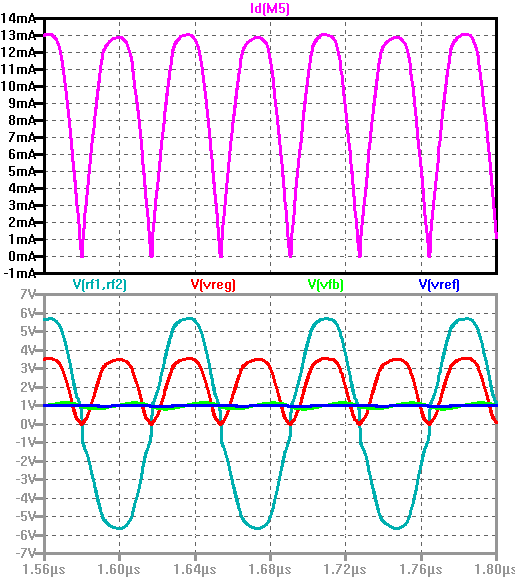
\includegraphics[width=\columnwidth]{Regulador_Sim_Hmax}
		\caption{\(H=H_{max}\)}
		\label{fig:ReguladorSimHmax}
	\end{subfigure}
	\quad
    \begin{subfigure}[b]{0.48\textwidth}
	    \centering
		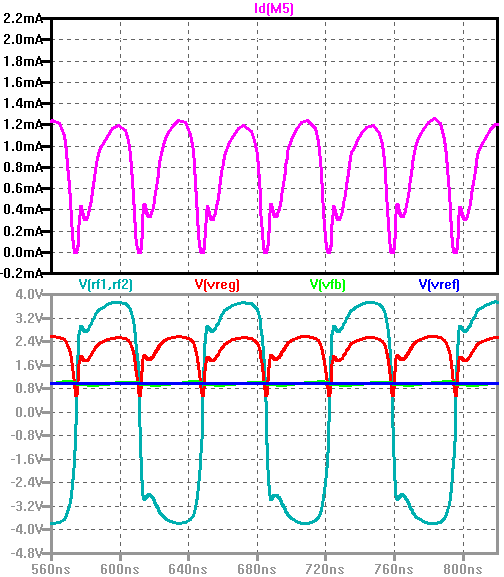
\includegraphics[width=\columnwidth]{Regulador_Sim_Hmin}
		\caption{\(H=H_{min}\)}
		\label{fig:ReguladorSimHmin}
	\end{subfigure}
	\caption{Simulación del regulador de tensión en funcionamiento. 
	Arriba se muestra la corriente a través del regulador de paso. 
	Abajo las tensiones en la antena, \(V_{reg}\), \(V_{fb}\) y 
	\(V_{ref}\).}
	\label{fig:ReguladorSim}
\end{figure}

Con campo máximo el regulador consume una corriente pico de 
\SI{13}{\milli\ampere}, se tienen \SI{3.5}{\volt} de tensión pico 
sobre el transistor de paso y una tensión inducida en la antena de 
\SI{5.5}{\volt} pico, lo que da una caída máxima de \SI{2}{\volt} en 
el rectificador. En estas condiciones el valor medio de \(V_{reg}\) es 
de \SI{2.2}{\volt} y \(V_{fb}\) es aproximadamente igual a \(V_{ref}\) 
lo que implica que el lazo de realimentación funciona correctamente.

Con campo mínimo, la corriente derivada por el regulador es de poco más
de \SI{1}{\milli\ampere}, mientras que la tensión inducida en la 
antena es de \SI{4}{\volt} pico y \(V_{reg}\) es \SI{2.5}{\volt} pico. 
Si bien en esta situación el regulador no debería derivar corriente a 
\emph{ground}, ya que el valor medio de \(V_{reg}\) está por debajo de 
\SI{2.2}{\volt}, que eso suceda no afectaría en principio el 
funcionamiento del transponder ya que la tensión inducida en la antena 
es de \SI{4}{\volt} pico y es suficiente para alimentar al dispositivo.


\subsection{Rectificador + Filtro}

En la figura \ref{fig:RectificadorFiltro} se muestra el circuito 
implementado dentro del bloque <<Rectificador + Filtro>>. Los puertos 
\(rf_{1}\) y \(rf_{2}\) son los terminales de entrada de la antena, al 
igual que en la figura \ref{fig:ReguladorCircuito} donde se muestra 
el circuito del regulador. Se tiene un segundo rectificador del 
mismo tipo que el de la figura \ref{fig:Rectificador}, pero con 
dispositivos de mucho menor tamaño, y un capacitor implementado con 
un transistores PMOS trabajando en acumulación y capacidades 
parásitas entre capas de metal. La salida \(V_{dd}\) es la tensión 
de alimentación general para todo el circuito integrado. Allí se 
conecta el bloque digital, el detector de pausas, el circuito generador 
de reloj, el \emph{power--on reset} y el regulador. 

\begin{figure}
	\centering
	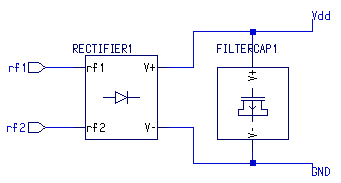
\includegraphics[width=0.5\columnwidth]{Rectificador_filtro}
	\caption{Circuito Rectificador + Filtro.}
	\label{fig:RectificadorFiltro}
\end{figure}

La tensión de alimentación \(V_{dd}\) no es más que la señal portadora 
recibida en la antena rectificada y filtrada, y su valor varía con la 
tensión pico inducida en la antena. Por otro lado, cuando el lector 
transmite información lo hace generando pausas de aproximadamente 
\SI{2.36}{\micro\second} en la portadora, por lo 
que la energía recibida se debe almacenar para ser usada durante los 
intervalos en que el dispositivo no recibe alimentación. Para ello el 
capacitor de filtrado tiene que tener una capacidad tal que la tensión 
\(V_{dd}\) no caiga por debajo de la tensión mínima requerida para que 
la lógica mantenga su estado. Si bien no se recibe energía durante 
las pausas, es precisamente en esos momentos en que el dispositivo 
consume la mínima energía debido a que también se detiene la señal 
de reloj y por lo tanto el bloque digital está en estado estático y 
sin consumo dinámico.

Para dimensionar tanto el rectificador como el capacitor de filtro se 
debe conocer cuál es el consumo de corriente de los bloques conectados 
a ellos. Por simulación se obtuvo el consumo promedio del bloque 
digital, que es de \SI{325}{\micro\ampere} cuando tiene señal de reloj 
aplicada y se lo alimenta con \SI{3.5}{\volt}; y menor a 
\SI{1}{\nano\ampere} sin señal de reloj. El otro 
circuito que su consumo depende del reloj es el generador de reloj 
propiamente dicho, ya que cuenta con compuertas lógicas y cambia de 
estado al ritmo de la portadora. Su consumo dinámico es de casi 
\SI{100}{\micro\ampere} y el estático es despreciable al igual que el 
del bloque digital. Los circuitos restantes apenas 
consumen \SI{13}{\micro\ampere}, por lo tanto el consumo total es de 
\SI{440}{\micro\ampere} con reloj y considerando un peor caso puede 
tomarse un valor de \SI{15}{\micro\ampere} sin reloj.

\begin{table}
	\centering
	\begin{tabu} to 0.9\columnwidth {X[l]X[c]X[c]}
		\toprule
		~ & \multicolumn{2}{c}{Consumo a \(V_{dd}=\SI{3.5}{\volt}\)}\\
		Bloque & En Pausas & Con Portadora \\
		\midrule
		Digital & \(<\SI{1}{\nano\ampere}\) & \SI{325}{\micro\ampere} \\
		Generador de Reloj & \(<\SI{1}{\nano\ampere}\) & \SI{100}{\micro\ampere} \\
		\emph{Power--on reset} & \SI{3}{\micro\ampere} & \SI{3}{\micro\ampere} \\
		Ref. de Corriente & \SI{6}{\micro\ampere} & \SI{6}{\micro\ampere} \\
		Amplificador & \SI{2}{\micro\ampere} & \SI{2}{\micro\ampere} \\
		Detector de Pausas & \SI{2}{\micro\ampere} & \SI{2}{\micro\ampere} \\
		\midrule
		Total & \SI{13}{\micro\ampere} & \SI{438}{\micro\ampere} \\
		\bottomrule
	\end{tabu}
	\caption{Corrientes promedio consumidas por los bloques que toman 
	su alimentación de \(V_{dd}\).}
	\label{tab:ConsumoPorBloque}
\end{table}

Entonces se deben analizar dos casos: Cuando el transponder recibe la 
señal portadora y la lógica CMOS está cambiando de estado; y cuando se 
está en el intervalo de \emph{pausa}, con los bloques digitales 
estáticos.

En el primer caso, y a los fines de considerar sólo la carga 
promedio, el consumo dinámico de la lógica se puede modelar como una 
resistencia. Además, si sumamos las corrientes del bloque digital 
más la del generador de reloj, el consumo de los bloques restantes 
---que no es de tipo resistivo ya que esos bloques contienen fuentes de 
corriente--- es despreciable. Por lo tanto la carga total es 
equivalente a un resistor de \SI{10}{\kilo\ohm} conectado en 
paralelo con el capacitor de filtrado. 

El \emph{ripple} para un rectificador de onda completa con capacitor 
de filtrado y carga resistiva puede calcularse según la siguiente 
ecuación:

\begin{equation*}
	V_{ripple} = \frac{V_{p}}{R_{L} C_{f}} \cdot \mathrm{T}
\end{equation*}

Donde \(V_{p}\) es la tensión pico a la salida del rectificador, 
\(R_{L}\) es la resistencia de carga, \(C_{f}\) la capacidad del 
capacitor de filtrado y \(\mathrm{T}\) el período de la onda 
senoidal rectificada. Suponiendo que queremos un \emph{ripple} menor 
al 10\% de la tensión de alimentación, se puede despejar de la 
ecuación la capacidad necesaria para lograrlo.

El peor caso para el cálculo del capacitor de filtrado se da 
cuando el transponder se encuentra lejos del lector, recibiendo la 
intensidad de campo mínima. En estas condiciones la tensión inducida 
en la antena es de \SI{4}{\volt} según se desprende de la figura 
\ref {fig:TensionInducida} para el caso RL, una inductancia de 
\SI{8}{\micro\henry} y \(R_{PICC}=\SI{10}{\kilo\ohm}\). Entonces, si 
se considera una caída de tensión de \SI{1.5}{\volt} en el 
rectificador, la tensión pico a la salida será de \SI{2.5}{\volt}. 
Además, la frecuencia de la onda senoidal rectificada es de 
\SI{27.12}{\mega\hertz} y por lo tanto su período es de 
\SI{36.8}{\nano\second}.

Haciendo las cuentas se llega a que la capacidad necesaria para 
obtener un \emph{ripple} menor al 10\% de \(V_{dd}\) es de 
\SI{36}{\pico\farad}.

\bigskip
Por otro lado, según la tabla \ref{tab:ConsumoPorBloque}, durante 
las pausas se tiene un consumo constante de \SI{13}{\micro\ampere} 
dado por los bloques \emph{Power-On Reset} (POR), la referencia de 
corriente, el amplificador y el detector de pausas. Estos bloques 
contienen fuentes de corriente y por lo tanto su consumo
es independiente de la tensión de alimentación. Por este motivo 
durante las pausas puede modelarse a la carga del capacitor de 
filtrado como una fuente de corriente que lo descarga de forma 
constante. La tensión en un capacitor con corriente constante varía 
de la siguiente forma:

\begin{equation}\label{eq:VcapConCorriente}
	V_{C} = \frac{1}{C} \cdot I \cdot t
\end{equation}

En el caso en que se tiene campo mínimo en la antena y por lo tanto 
\SI{2.5}{\volt} pico a la salida del rectificador, se puede tener como 
máximo una caída de tensión durante las pausas de \SI{1}{\volt}. De 
darse una caída de tensión de esa magnitud, la lógica 
digital quedaría alimentada con \SI{1.5}{\volt}, tensión más que 
suficiente para mantener el estado de los flip-flops.

Según el estándar, la duración de las pausas tiene un máximo de 
\SI{3}{\micro\second}, mientras que el consumo de corriente puede tomarse de 
\SI{15}{\micro\ampere} para tener algún margen de seguridad. Despejando
la capacidad de la ecuación para esos valores de tiempo y corriente, y 
para \SI{1}{\volt} de caída de tensión en \(V_{C}\) se obtiene 
\(C_{f}=\SI{45}{\pico\farad}\).

Resumiendo, la capacidad necesaria para que el circuito integrado se 
mantenga alimentado durante las pausas es de \SI{45}{\pico\farad}, 
mayor que la capacidad obtenida para tener un \emph{ripple} de 
tensión del 10\%. Es evidente que cuanto mayor sea la capacidad 
menor será el \emph{ripple} y menor será la caída de tensión durante 
las pausas en la portadora. Por lo tanto, en la implementación del 
diseño el capacitor de filtrado tendrá que ser de al menos 
\SI{45}{\pico\farad}, pero podría ser mayor si hubiese espacio 
sobrante dentro del \emph{die}.

\bigskip
Para finalizar, la implementación del capacitor de filtrado 
se realizó con transistores PMOS, ya que estos ofrecían la mayor 
capacidad por unidad de superficie (\SI[per-mode=symbol]{2.474}{
\femto\farad\per\micro\meter\squared} según la tabla 
\ref{tab:DatosProcesoCapacidades}). Se utilizaron varios 
transistores en paralelo y se conectó el terminal de \emph{gate} de 
cada uno de ellos a \(V_{dd}\) y sus \emph{bulks}, formados por 
difusiones tipo N a \(GND\). De esta forma se obtuvo un capacitor MOS 
formado entre la capa de \emph{poly} y el \emph{Nwell} y se lo hizo 
trabajar en acumulación, modo en que la capacidad por unidad de área 
es constante y no depende de la tensión aplicada.

Para aumentar la capacidad de la estructura también se aprovechó la 
capacidad existente entre la capa de metal 
más baja (M1) y el poli-silicio, utilizando el conexionado de la 
figura \ref{fig:CapacitoresMOS}. Se conectaron un total de 27 
dispositivos de \(\SI{40}{\micro\meter} \times \SI{40}{\micro\meter}\) 
en el área no utilizada del chip y se trazaron tiras de M1 sobre 
ellos, conectando todo el conjunto como indica la figura, y logrando una 
capacidad teórica de aproximadamente \SI{100}{\pico\farad}.

\begin{figure}
	\centering
	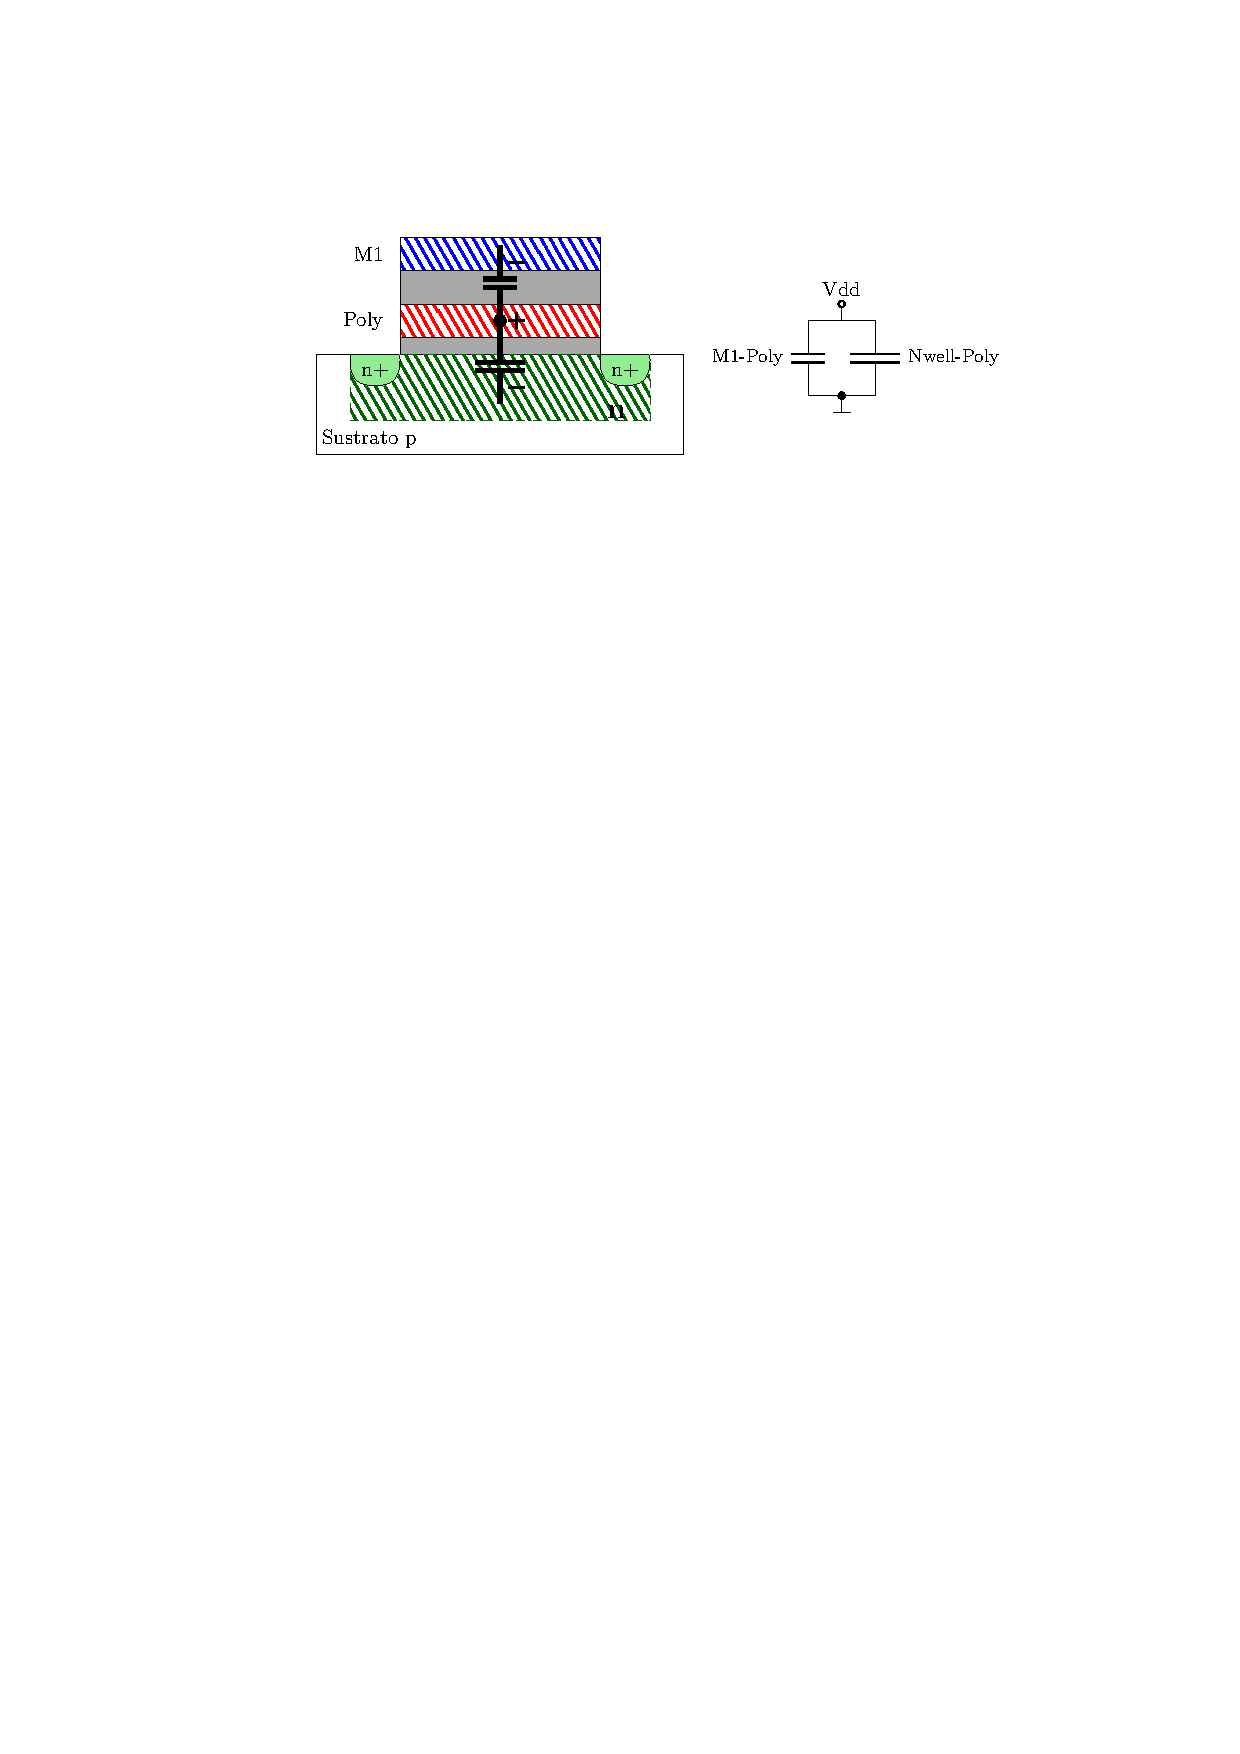
\includegraphics[]{CapacitorPMOS}
	\caption{Capacitor de filtrado implementado con capacitores MOS y 
	la primer capa de metal.}
	\label{fig:CapacitoresMOS}
\end{figure}


\section{Transmisión y recepción de datos}

Los bloques analógicos involucrados en la transmisión y recepción de 
datos traducen la información recibida del dominio analógico al 
digital y vice-versa. Por un lado en la recepción de datos de deben 
detectar las pausas introducidas por el lector en la señal portadora 
y generar la señal \lstinline{pause} (ver figura 
\ref{fig:DecodedReception}) que deberá ingresar al sistema digital. 
Por el otro, en la transmisión hacia el lector se debe realizar la 
modulación de carga sobre la señal portadora según la información 
codificada por el sistema digital en \lstinline{coded_out} (figura 
\ref{fig:BitCoderDiagBloques}).

\subsection{Detector de Pausas}

En la figura \ref{fig:PauseDetectorCircuit} se muestra el circuito 
propuesto para el detector de pausas. Los puertos \emph{rf1} y 
\emph{rf2} son la entrada de la tensión de la antena, \emph{Vpos} es 
la tensión de alimentación interna, a través de \emph{Irefn\_in} 
ingresa una corriente de referencia de \SI{1}{\micro\ampere} y en 
\emph{Pause} se obtiene la señal para el bloque digital.

\begin{figure}
	\centering
	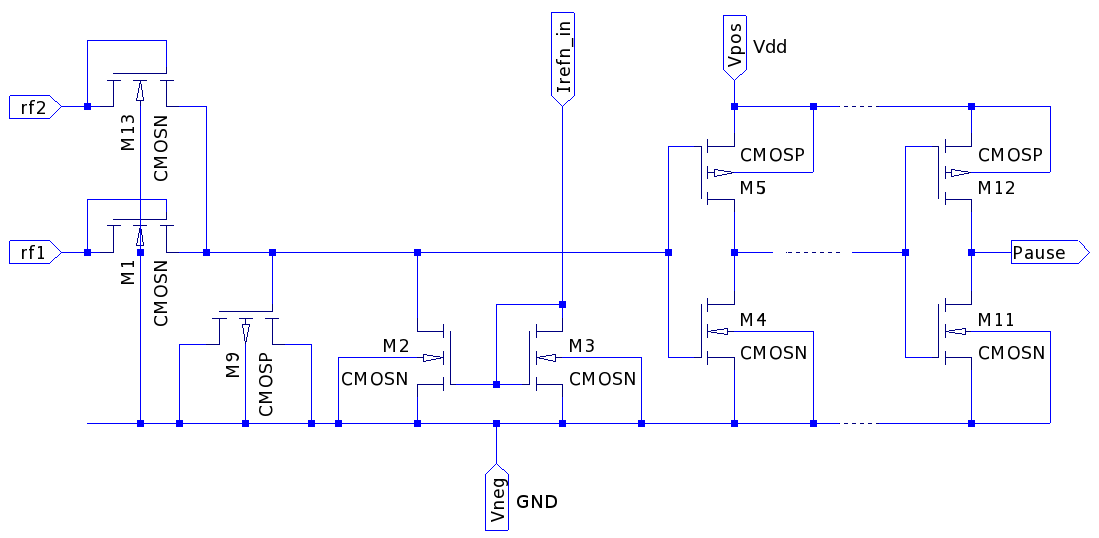
\includegraphics[width=\columnwidth]{PauseDetector_circuit}
	\caption{Circuito detector de pausas.}
	\label{fig:PauseDetectorCircuit}
\end{figure}

La tensión entre \emph{rf1} y \emph{rf2} es la tensión inducida en 
la antena y por lo tanto su forma de onda es senoidal. Sin embargo, 
tomando las tensiones de esos nodos contra GND se obtienen 
dos medias ondas rectificadas desfasadas \SI{180}{\degree} una de 
otra, ya que, como se observa en la figura \ref{fig:RectificadorFiltro},
de esa forma se toma la tensión entre la entrada y la salida del 
rectificador. 

Los transistores M1 y M13 están conectados como diodos y forman 
la parte positiva de un rectificador de onda completa. M9 hace de 
capacitor MOS y se carga con las corrientes provenientes de la 
entrada de RF, mientras que M2 y M3 forman una fuente de corriente 
espejo que lo descarga a corriente constante. Luego se tiene una 
cadena de inversores que cambian de estado según la tensión de M9 y 
amplifican la variación de tensión de forma tal de tener flancos 
abruptos en \emph{Pause}.

En la figura \ref{fig:PauseDetectorSim} se observa una simulación 
del circuito en funcionamiento. Allí se observa como el capacitor se 
encuentra cargado a la tensión máxima y al producirse la pausa se 
descarga de forma lineal con la fuente de corriente. Cuando la tensión 
en ese nodo es menor que \(\sfrac{V_{dd}}{2}\) los inversores cambian 
de estado y \emph{Pause} pasa de 1 a 0. Al finalizar la pausa y 
regresar la portadora el capacitor se carga nuevamente en los primeros 
ciclos de la señal, haciendo que la salida vuelva a su estado 
original. 

\begin{figure}
	\centering
	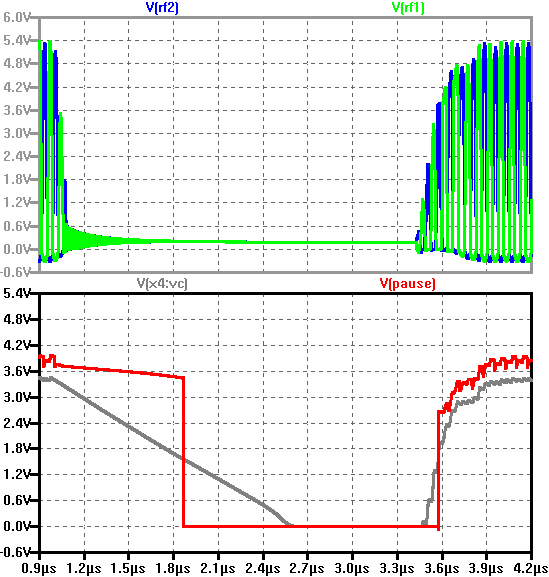
\includegraphics[width=0.6\columnwidth]{PauseDetector_Sim}
	\caption{Simulación del circuito detector de pausas.}
	\label{fig:PauseDetectorSim}
\end{figure}

Para el cálculo del capacitor se consideró que se debía descargar 
con una corriente de \SI{1}{\micro\ampere} desde la tensión máxima 
inducida en la antena hasta cero en \SI{1.5}{\micro\second}, es 
decir, en la mitad del tiempo de la pausa. Usando la fórmula de la 
tensión en un capacitor con corriente constante 
\eqref{eq:VcapConCorriente} se obtuvo que la capacidad necesaria es de 
\SI{500}{\femto\farad}.

El capacitor fue implementado con un transistor PMOS en acumulación, 
al igual que los capacitores de filtrado de \(V_{dd}\). De la 
información del proceso se tiene que la capacidad entre las capas de 
\emph{Nwell} y \emph{poly} en la zona activa es de 
\SI[per-mode=symbol]{2.474}{\femto\farad\per\micro\meter\squared} y 
por lo tanto se trazó un transistor PMOS de 
\(15\times15\)\si{\micro\meter}.

\begin{figure}
	\centering
	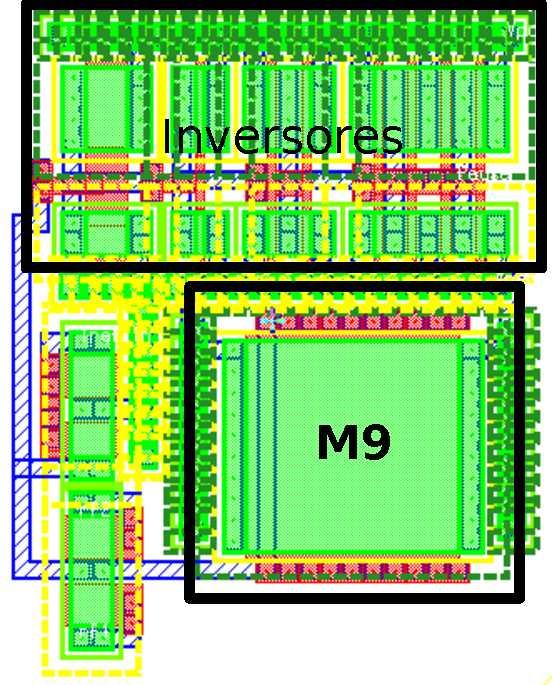
\includegraphics[width=0.4\textwidth]{Layout_PauseDetector.pdf}
	\caption{\emph{Layout} del detector de pausas.}
	\label{fig:PauseDetectorLayout}
\end{figure}

\subsection{Modulador}
\label{sec:Modulador}

El bloque modulador es el encargado de realizar la modulación de carga 
sobre la antena para transmitir la información hacia el lector. Como 
se vio en la sección \ref{sec:InterfIndTransDatos} existen dos 
formas de realizar la modulación: Resistiva y Capacitiva. En este caso 
se decidió utilizar una carga capacitiva.

En la figura \ref{fig:ModulatorCircuit} se muestra el bloque 
modulador. Se trata de un diseño simple que conecta/desconecta los 
capacitores C1 y C2 a la antena y estos actúan de carga. Los 
transistores M1 y M2 actúan de llaves comandadas por la señal 
\lstinline{coded_out} del bloque modulador digital de la figura 
\ref{fig:BitCoderDiagBloques}.

\begin{figure}
	\centering
	\begin{subfigure}[b]{0.4\textwidth}
		\centering
		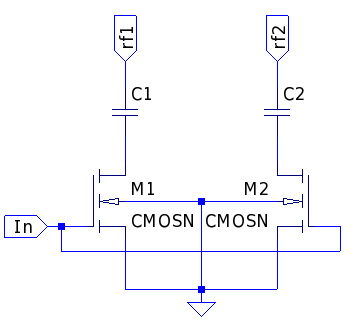
\includegraphics[width=\columnwidth]{Modulator_circuit}
		\caption{Esquemático.}
		\label{fig:ModulatorCircuit}
	\end{subfigure}
	\quad
    \begin{subfigure}[b]{0.4\textwidth}
	    \centering
		\raisebox{-0.5\height}{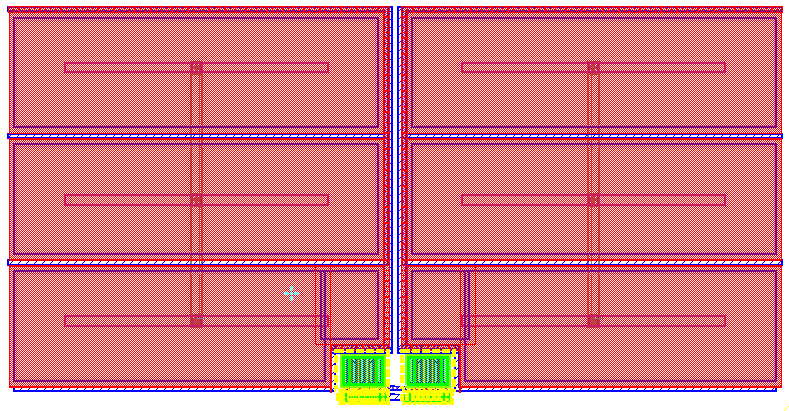
\includegraphics[width=\columnwidth]{Layout_Modulator}}
		\caption{Layout.}
		\label{fig:ModulatorLayout}
	\end{subfigure}
	\caption{Circuito modulador de la señal portadora.}
	\label{fig:ModulatorCircuitLayout}
\end{figure}

En la figura \ref{fig:ModulatorCircuitSim} se muestra una simulación 
del funcionamiento del circuito modulador. Allí se observan las 
tensiones en los capacitores C1 y C2 y la señal de encendido de las 
llaves. Cuando la señal \lstinline{coded_out} está en cero las llaves se 
encuentran abiertas y por lo tanto no circula corriente por los 
capacitores. Este es el estado \emph{descargado} de la señal 
portadora. Por otro lado, cuando \lstinline{coded_out} es igual a 
\((V_{dd}\) se cierran las llaves y C1 y C2 quedan conectados a la 
antena actuando como cargas. En este caso se dice que la portadora se 
encuentra \emph{cargada}. Durante el semiciclo positivo 
de \emph{rf1} la corriente circula a través de C1 y en el 
semiciclo positivo de \emph{rf2} la corriente circula a través de 
C2, es decir, los capacitores y la llaves trabajan de forma 
alternada debido a que las tensiones de la entrada de la antena 
respecto de GND se ven como medias ondas rectificadas. 

\begin{figure}
	\centering
	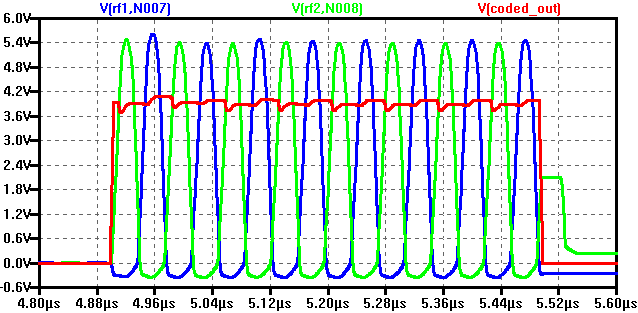
\includegraphics[width=0.6\columnwidth]{Modulator_sim}
	\caption{Simulación del circuito modulador de la señal portadora. 
	Los trazos verde y azul son las tensiones en C1 y C2 
	respectivamente, mientras que el trazo rojo es la señal de comando 
	formada por los datos modulados con la sub-portadora.}
	\label{fig:ModulatorCircuitSim}
\end{figure}

Los capacitores fueron implementados con las capas \emph{poly-poly2} 
debido a que era necesario conectar ambos terminales a nodos 
distintos de GND y eso no hubiese sido posible con otro tipo de 
capacitores.

El estándar da un límite mínimo para la amplitud de la modulación de 
carga medida con el arreglo ISO/IEC 10373--6 de \SI{18}{\milli\volt} 
pico con \(H_{\text{mín}}\) y \SI{9}{\milli\volt} pico con \(
H_{\text{máx}}\) (figura \ref{fig:AmplitudesPICC_PCD}). De la figura 
\ref{fig:VsensModulacionC} y el análisis relacionado se desprende que
con una capacidad de \SI{8}{\pico\farad} debería obtenerse una 
modulación de amplitud suficiente. 

Los capacitores de \emph{poly-poly2} tienen una capacidad de 
\SI[per-mode=symbol]{0.885}{\femto\farad\per\micro\meter\squared}, por 
lo tanto es necesaria un área de \(95\times95\si{\micro\meter}\) para 
cada uno de ellos. El trazado físico final del bloque puede verse en la 
figura \ref{fig:ModulatorLayout}.


\section{Generador de reloj}

El generador de reloj se encarga de producir la señal de reloj 
necesaria para el sistema digital. Esta señal debe ser de exactamente 
la misma frecuencia que la portadora debido a que el sistema digital 
depende de esta base de tiempo para codificar y decodificar la 
información. Además debe contar con flancos rápidos, de muy corta 
duración, para disminuir el consumo dinámico de la lógica CMOS, y no 
debe contener \emph{glitches} que puedan llevar al sistema digital a 
un estado indeseado.

En la figura \ref{fig:ClockGeneratorCircuit} se muestra el esquema 
eléctrico del generador de reloj. Para obtener una señal de la misma 
frecuencia que la portadora se decidió generarla a partir de la 
portadora misma. 

\begin{figure}
	\centering
	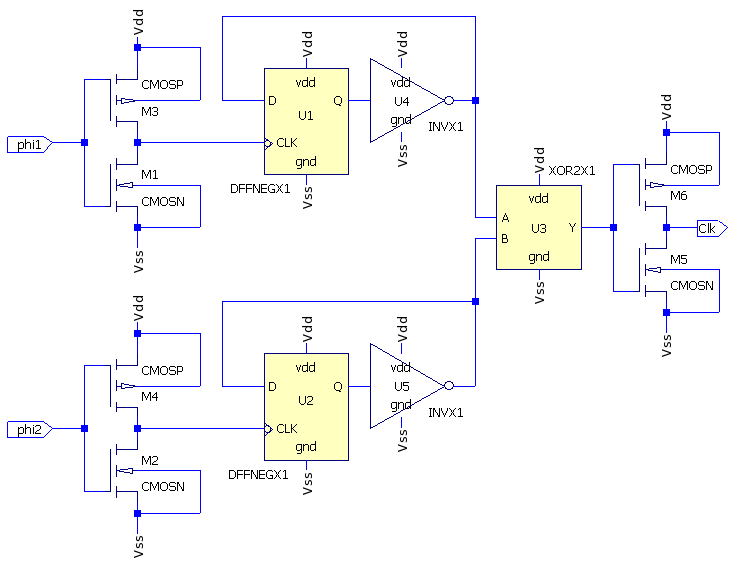
\includegraphics[width=0.8\columnwidth]{ClockGenerator_circuit}
	\caption{Esquema eléctrico del bloque generador de reloj.}
	\label{fig:ClockGeneratorCircuit}
\end{figure}

Las entradas \emph{phi1} y \emph{phi2} están conectadas a las entradas 
provenientes de la antena \emph{rf1} y \emph{rf2}, por lo que se 
tienen allí tensiones de tipo senoidal media onda rectificada, 
desfasadas \SI{180}{\degree} entre ellas. Luego se tienen dos 
inversores desbalanceados para obtener el punto de cambio de estado 
más cerca de \(V_{dd}\) que de cero. Estos inversores convierten la 
entrada de RF en señales cuadradas que disparan un par de flip-flops 
T, que cambian de estado con cada flanco descendente de reloj. Las
salidas de los flip-flops son dos señales cuadradas de la mitad de 
frecuencia que la portadora desfasadas \SI{90}{\degree}, como se 
muestra en la simulación de la figura \ref{fig:ClockGeneratorSim}. La 
señal de reloj se obtiene a partir de la operación XOR de las salidas 
de los flip-flops y para poder manejar la carga del conexionado y la 
entrada del árbol de reloj del bloque digital se agregó un inversor 
del doble del tamaño del inversor mínimo.

\begin{figure}
	\centering
	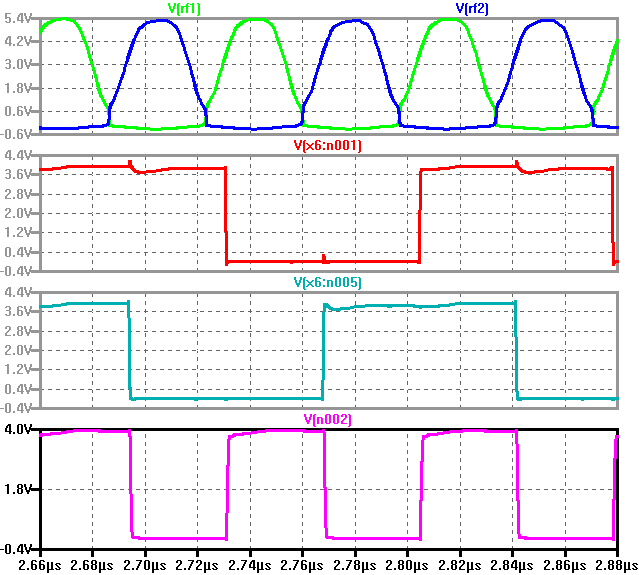
\includegraphics[width=0.65\columnwidth]{ClockGenerator_sim}
	\caption{Simulación del bloque generador de reloj.}
	\label{fig:ClockGeneratorSim}
\end{figure}

La señal de reloj producida por este método es obtenida a partir del 
período de la señal portadora y por lo tanto tiene su misma 
frecuencia y además está sincronizada con ella. Al producirse una 
pausa, la amplitud de las tensiones en \emph{rf1} y \emph{rf2} se reduce 
de forma monótona hasta llegar a cero (este es un requisito que debe 
cumplir la portadora según el estándar). Cuando dicha 
amplitud es menor que la tensión umbral de los inversores de 
entrada los flip-flops quedan detenidos en un estado y lo mismo sucede 
con el reloj. 

Al finalizar la pausa, en principio no se sabe que entrada, \emph{phi1} 
o \emph{phi2}, hará que el correspondiente flip-flop cambie 
de estado. Sin embargo esto no es un problema ya que como el reloj 
es resultante de la operación XOR, no importa que cambie la fase de 
sus entradas, la salida seguirá siendo una señal cuadrada y no 
contendrá el cambio de fase de la entrada. Por ejemplo, si durante la 
pausa las entradas de la XOR quedan en los estados A=`0' y B=`1', dados 
por los correspondientes FFs U1 y U2, la salida 
de reloj se mantendrá en estado `0'. Si al retornar la portadora el 
primer FF cambia de estado y la entrada A de la XOR pasa de `0' a `1', 
entonces la salida de reloj cambiará al estado `1'. Si por el 
contrario U2 cambiase de estado primero al retornar la portadora, 
entonces la entrada B de la XOR pasará a `0', mientras que A se 
mantendrá en `0', y entonces la salida de reloj también cambiará al 
estado `1'. 


\section{\emph{Power-On Reset} (POR)}

Cuando el dispositivo es acercado a la zona de influencia de un 
lector, se induce una tensión en la antena y la alimentación interna 
crece de cero al nivel máximo en algunos milisegundos (Recordar que el 
campo del lector está siempre activo y es el transponder el que es 
acerca. Cuanto tarda la tensión en llegar al nivel de operación 
dependerá de que tan rápido se aproxime). 
El bloque \emph{power-on reset} se encarga de generar la señal 
\lstinline{reset} para el sistema digital cuya función es llevarlo 
al estado inicial en el arranque del dispositivo. En la figura 
\ref{fig:PORCircuit} se muestra el esquema eléctrico del POR, cuyo 
diseño está basado en el presentado en \cite{Gudnason}.

\begin{figure}
	\centering
	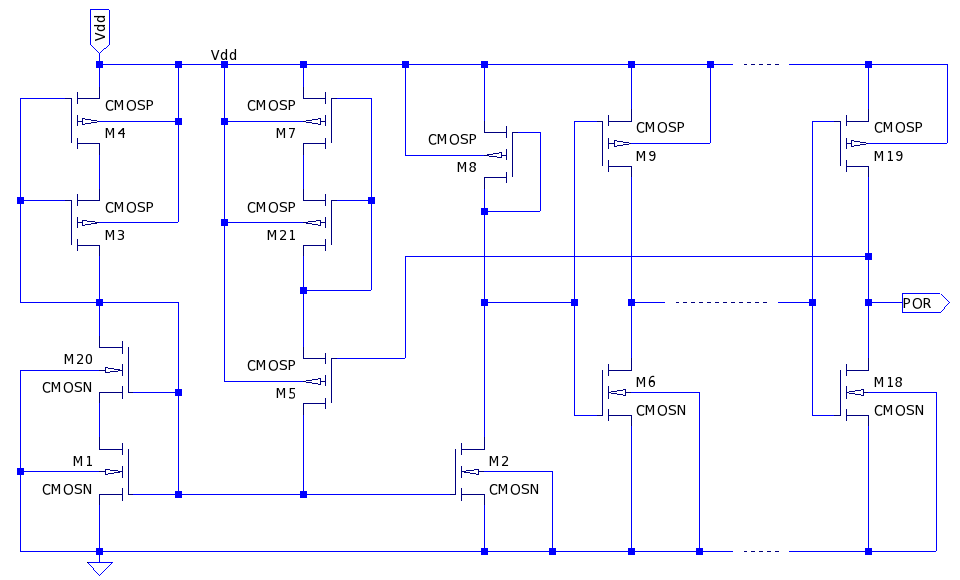
\includegraphics[width=\columnwidth]{POR_circuit}
	\caption{Esquema eléctrico del bloque \emph{power-on reset}.}
	\label{fig:PORCircuit}
\end{figure}

Su funcionamiento se basa en la comparación de las corrientes que 
circulan por dos transistores de tamaños diferentes para así liberar 
la señal \lstinline{reset} cuando \(V_{dd}\) alcanza la tensión de 
funcionamiento.

Cuando \(V_{dd}\) está por debajo de la tensión mínima de operación 
\(V_{dd_{\text{mín}}}\), no circula corriente por M2 y por lo tanto M8 
conecta la entrada de la cadena de inversores a \(V_{dd}\), haciendo 
que la salida \lstinline{POR} se encuentra en alto. A su vez el 
transistor M5, que actúa como llave, se encuentra cortado.

Al superar \(V_{dd}\) a \(V_{tn}+V_{tp}\) comienza 
a circular una corriente a través de M1-20, M3-4 que depende de \(
V_{dd}\) de forma cuadrática, ya que esos transistores están 
conectados como diodos. M2 copia esta corriente y la hace circular a 
través de M8, que es un transistor más largo que ancho y tiene un 
\emph{beta} menor que M3-4. Entonces, al ir aumentando \(V_{dd}\) la 
corriente requerida por la fuente de corriente espejo a través de M2 
superará a la que puede entregar M8 para la misma tensión de 
alimentación y por lo tanto la tensión del nodo intermedio pasará de 
\(V_{dd}\) a cero, haciendo que cambie el estado de la salida.

En la figura \ref{fig:PORCorrientes} el drain de M2 fue conectado a 
\(V_{dd}\) y el drain de M8 a GND. Allí se ve como la corriente a 
través de M2 crece de forma cuadrática una vez superada la tensión 
\(V_{tn}+V_{tp}\) y como la corriente a través de M8 comienza a crecer 
antes, pero con un \emph{beta} menor. Cuando se supera el punto de 
cruce la caída de tensión en M8 aumenta y por lo tanto el drain de M2 
cae, haciendo que la cadena de inversores cambie de estado y la señal 
\lstinline{POR} sea cero.

\begin{figure}
	\centering
	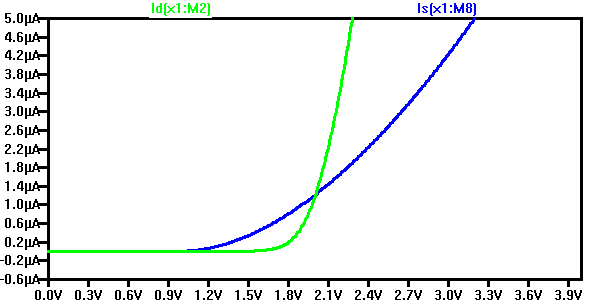
\includegraphics[width=0.6\columnwidth]{POR_corrientes}
	\caption{\(I_{D2}\) e \(I_{D8}\) en función de la tensión de 
	alimentación. En esta simulación los drains de M2 y M8 
	fueron conectados a \(V_{dd}\) y \(GND\) respectivamente.}
	\label{fig:PORCorrientes}
\end{figure}

M5 y M7-21 agregan una pequeña histéresis al circuito. Cuando 
\lstinline{POR} pasa al estado cero, M5 conecta a M7-21 en paralelo 
con M3-4, aumentando el ancho efectivo del transistor equivalente. 
Esto hace que circule mayor corriente a través de M1-20 y, a través 
de la copia espejo, la caída en M8 aumente aún más. De esta forma se 
evita que la salida del circuito quede oscilando cuando \(V_{dd}\) 
alcanza el límite de la transición.

En a figura \ref{fig:PORTensiones} se observa la tensión del drain 
de M2 junto con la salida a medida que aumenta \(V_{dd}\).

\begin{figure}
	\centering
	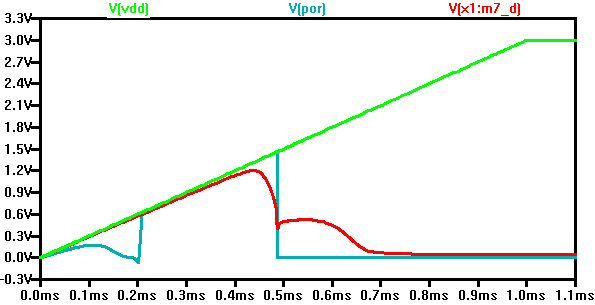
\includegraphics[width=0.6\columnwidth]{POR_Sim}
	\caption{Tensión del drain de M2 y de salida del circuito cuando 
	\(V_{dd}\) aumenta de cero a \SI{3}{\volt}.}
	\label{fig:PORTensiones}
\end{figure}
